\documentclass{article}
\usepackage{amsmath}
\usepackage{commath}
\usepackage{graphicx}

\renewcommand{\thesection}{\arabic{section}.}
\renewcommand{\thesubsection}{(\alph{subsection})}

\pagestyle{empty}

\begin{document}
\section{}
\subsection{}
Take the total differentiation of the LM-IS equation and we obtain the following set of linear equation:
\[
    \begin{pmatrix}
        C' - 1 & I' \\
        P L_Y & P L_r
    \end{pmatrix}
    \begin{pmatrix}
        \dif Y \\ \dif r
    \end{pmatrix} =
    \begin{pmatrix}
        C' \dif T - \dif G \\
        \dif M - L \dif P
    \end{pmatrix},
\]
in which $L_Y \equiv \partial L / \partial Y$, $L_r \equiv \partial L / \partial r$.
Note that $\dif P = 0$ under the sticky-price assumption. Solving the equation set and we get that
\[
    \dif r = \frac{1}{P} \cdot
    \frac{(C' - 1) \dif M - P L_Y (C' \dif T - \dif G)}{L_r (C' - 1) - L_Y I'}.
\]
To keep the interest rate unchanged when $G$ increases by $\Delta G$, the central bank has to let $\dif r$ be zero. As for the central bank, $T$ is fixed. That is,
\begin{equation}
    \dif r = 0 \,\Longrightarrow\,
    (1 - C') \dif M = P L_Y \dif G. \label{eq1}
\end{equation}
Note that under our assumption, $C' < 1$ and $L_Y > 0$. Thus the central bank can increase money supply to maintain the interest rate.

\subsection{}
Solving the equation set in (a), we obtain
\[
    \dif Y = \frac{1}{P} \cdot
    \frac{P L_r (C' \dif T - \dif G) - I' \dif M}{L_r (C' - 1) - L_Y I'}.
\]
With the equation \eqref{eq1} and $\dif T = 0$, the government spending multiplier in this case is
\[
    \frac{\dif Y}{\dif G} = \frac{1}{1 - C'}.
\]

\section{}
\subsection{}
The model is
\begin{align*}
    Y &= C(Y - T) + I(r^\ast) + G + X(e, Y), \\
    \frac{M}{P} &= L(r^\ast, Y).
\end{align*}
The LM equation determains the output, which is a vertical line in the coordinate with $Y$ on the horizontal axis and $e$ on the vertical axis. For the IS equation, we can compute the derivatve
\[
    \frac{\partial e}{\partial Y} =
    - \frac{C' + X_Y - 1}{X_e} = \frac{(1 - C') - X_Y}{X_e}.
\]
Note that $0 < C' < 1$, $X_e < 0$ and $X_Y < 0$, which means $\partial e / \partial Y < 0$. Thus, the IS curve is downward-sloping in the coordinate.

When a fiscal stimulus is conducted (say, increasing the government expenditure), $Y$ should be larger given a fixed $e$. The IS curve shifts to the right and the LM curve does not change. Therefore, a fiscal stimulus results in a higher exchange rate and an unchanged output.

\subsection{}
The model is
\begin{align*}
    Y &= C(Y - T) + I(r^\ast) + G + X(e^\ast, Y), \\
    \frac{M}{P} &= L(r^\ast, Y).
\end{align*}
In this case, the endogenous variables are $Y$ and $M$. The IS curve is vertical in the coordinate with $Y$ on the horizontal axis and $M$ on the vertical axis. Under the assumption, $\partial M / \partial Y = P \cdot \partial L / \partial Y > 0$. Thus the LM curve is upward-sloping in the coordinate.

When there is a fiscal stimulus, the IS curve shifts to the right and the LM curve does not change. Therefore, a fiscal stimulus results in both larger output and larger money supply.

\section{}
\subsection{}
\begin{figure}[h]
    \centering
    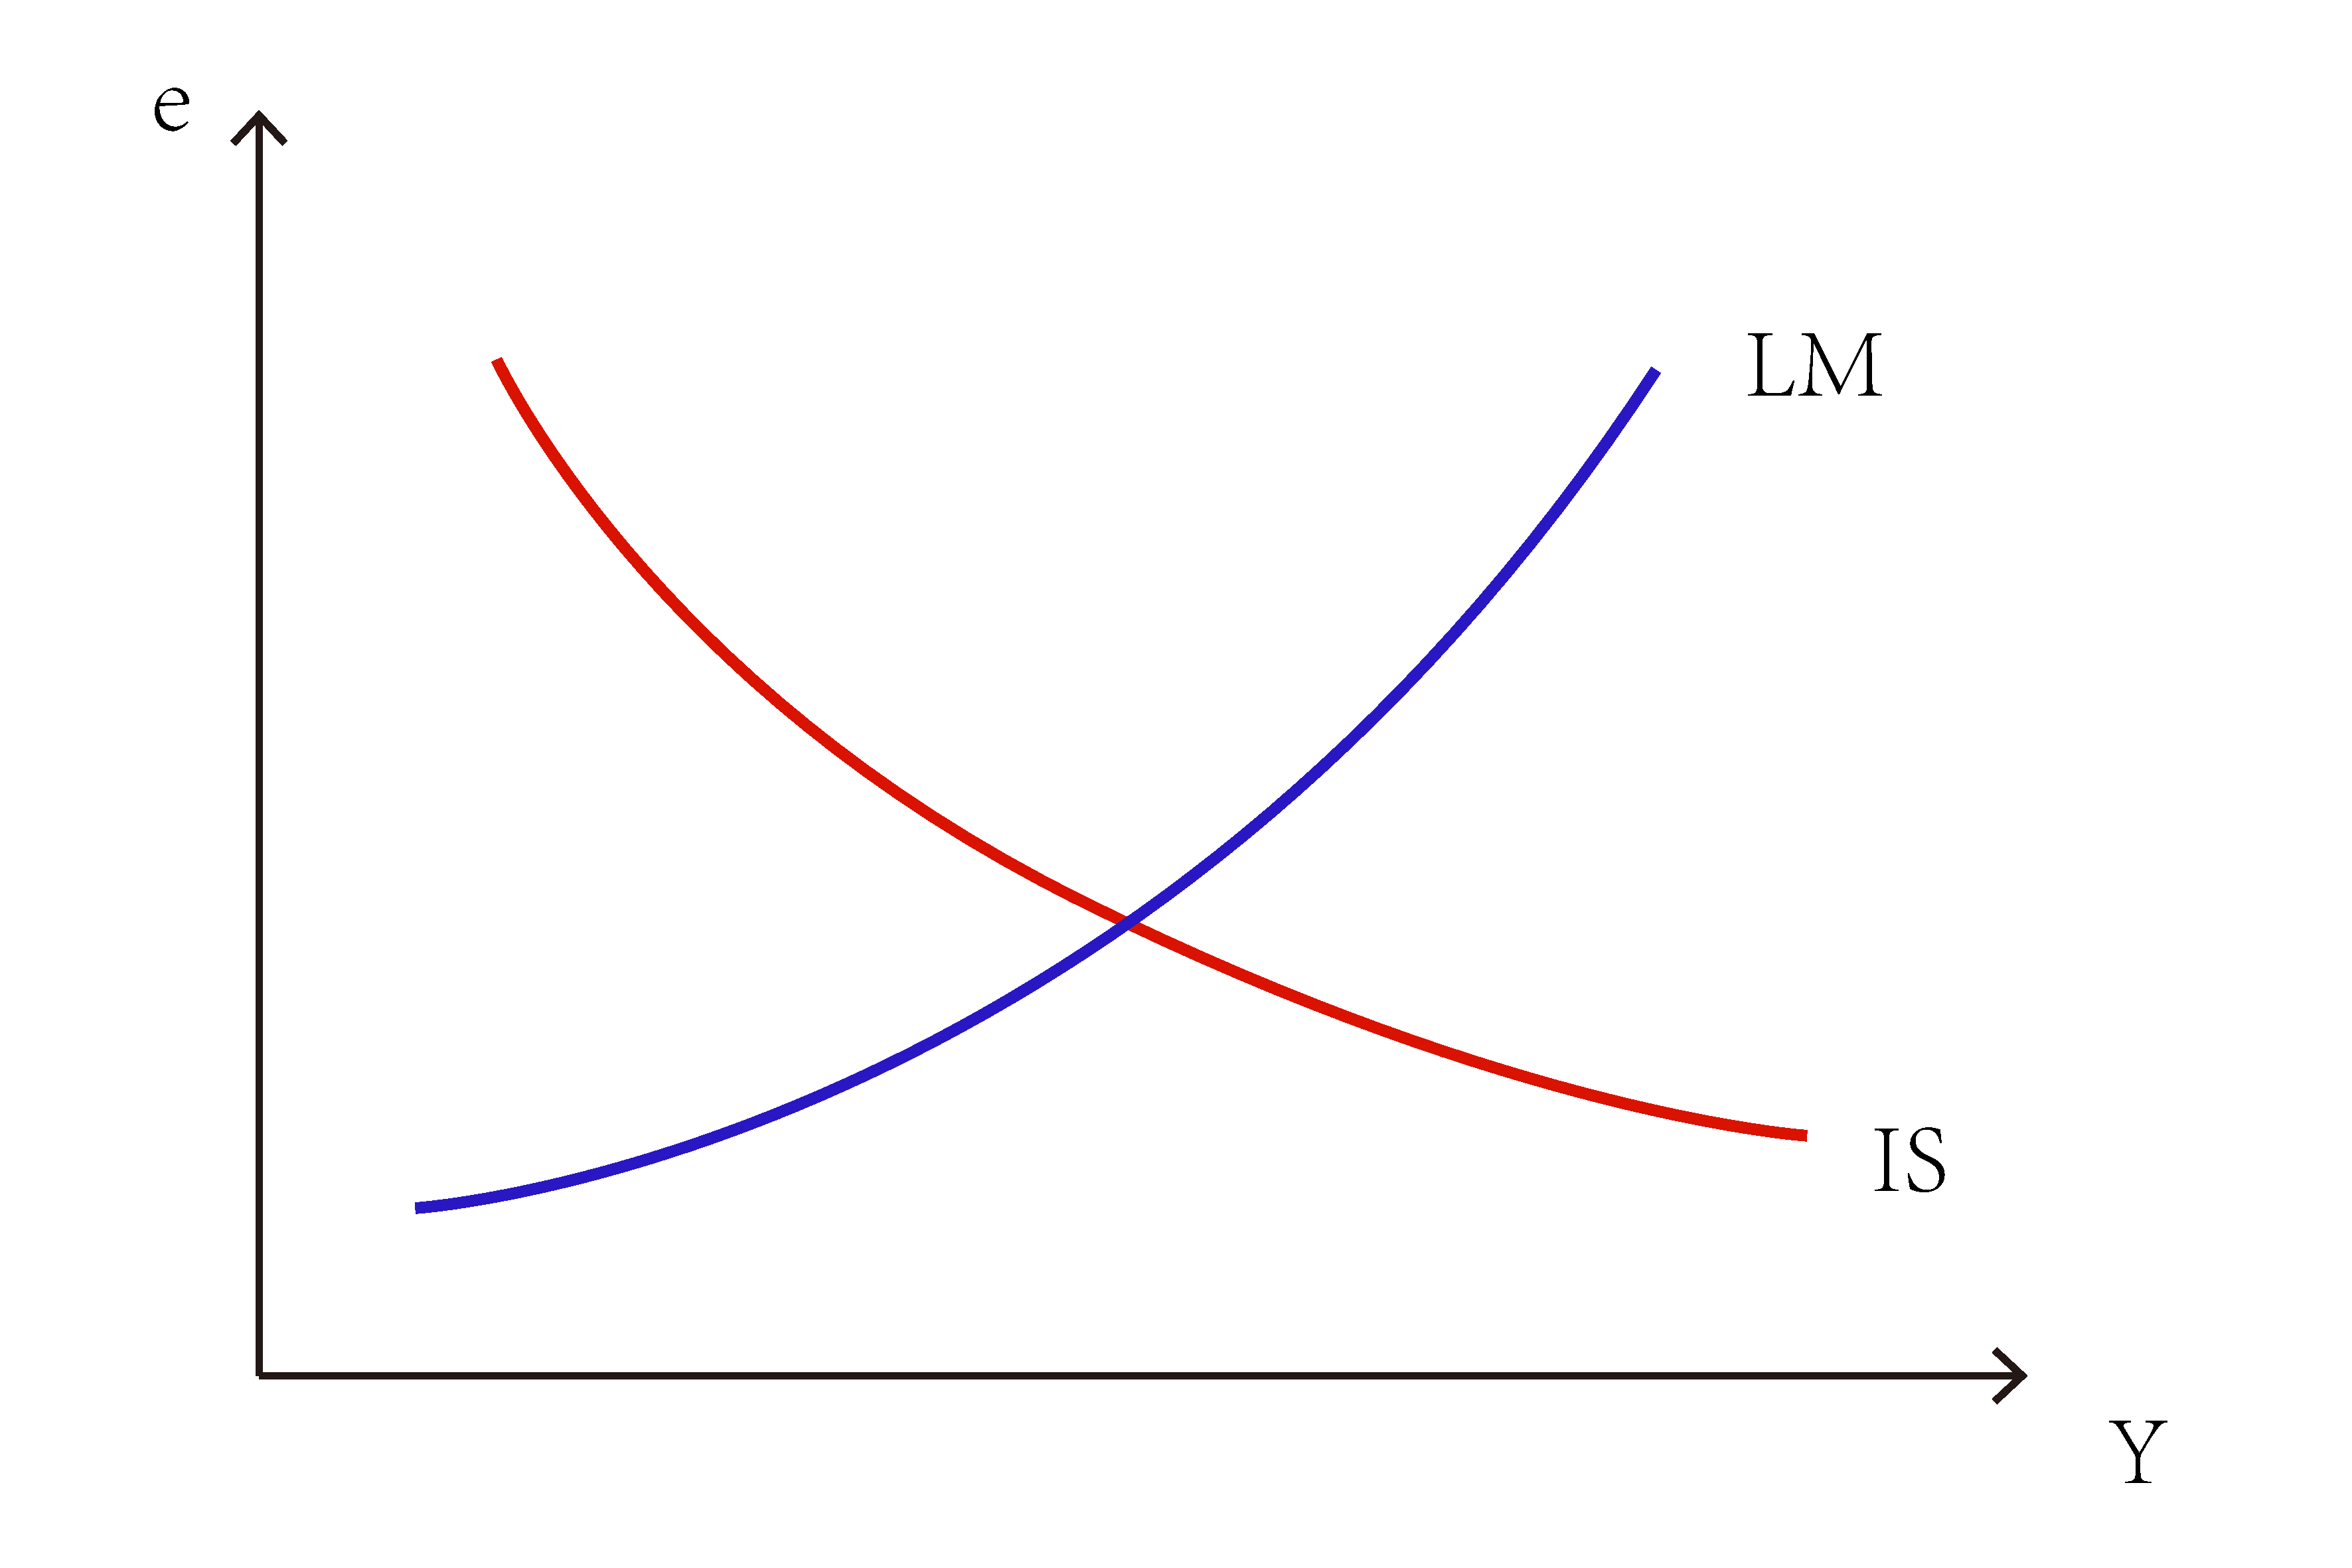
\includegraphics[scale=0.16]{Figure/figure.pdf}
    \caption{IS-LM curves}
    \label{fg1}
\end{figure}

\subsection{}
The model is
\begin{align*}
    Y &= C(Y - T) + I(r^\ast) + G + X(e), \\
    \frac{M}{P(e, w)} &= L(r^\ast, Y).
\end{align*}
When there is a negative foreign-demand shock, under the MPC-decreasing assumption,
\[
    \frac{\partial Y}{\partial X} =
    -\frac{1}{C' - 1} > 0.
\]
Therefore, the IS curve in Figure \ref{fg1} shifts to the left as for every $e$ the net export declines. This results in a lower output and a currency depreciation.

\subsection{}
Consider $w$ exogenous. The increase in domestic price means that for every $e$, $P(e, w)$ increases. Because
\[
    \frac{\partial Y}{\partial P} = - \frac{L}{P \cdot L_Y} < 0,
\]
the LM curve shifts to the left, resulting in the appreciation of the domestic currency and a lower output.

\end{document}